\documentclass[12pt,fleqn]{article}\usepackage{../../common}
\begin{document}
Materyel Mekaniği - 2

Sonsuz Küçük Gerilme Tensörü (Infinitesimal Strain Tensor)

Green gerilme tensörünü gördük, kuvvetli bir yaklaşım ama bizim daha çok
kullanacağımız şimdi anlatacağımız. Niye? Çünkü Green tensörü sonlu
deformasyonlar / yamulmalar için geçerli ama çoğu uygulamada bize lazım olan çok
ufak yamulmalar. Ufak derken, önceki dersteki (3) formülünden hareketle, oradaki
en son terimi hatırlarsak, çok ufak yamulmalar için $\nabla u^T \nabla u << \nabla u$ 
olur, yani ufak değişimlerde o karesel işlem $\nabla u$'dan daha ufak sonuç
verir. O zaman belli durumlarda son terim yaklaşık sıfır kabul edilebilir,
$\nabla u^T \nabla u \approx 0$. O zaman Green tensörü bu durumlarda yaklaşık
olarak alttaki gibi olur,

$$
\epsilon_{Green} \approx \frac{1}{2} (\nabla u + \nabla u^T )
$$

Bileşen formunda

$$
\epsilon_{ij} = \left(
\frac{\partial u_i}{\partial X_j} + \frac{\partial u_j}{\partial X_i}
\right)
$$

Bu tensör de simetrik, fakat sadece ufak şekil değişimleri, yamulmalar için
geçerli. Fakat zaten, mesela inşaat mühendisliği durumunda, binalar, demir
çubuklar (beam) ile iş yaptığımız zaman, bu tür şekil değişimi faraziyesi
yeterli. Çünkü eh, biraz düşünürsek eğer binamız büyük şekil değişimleri
yaşıyorsa önümüzde daha büyük bir problem var demektir.

Cauchy Stres Tensörü

Gerilme tensöründen stres tensörlerine geldik. İlk önce çekiş (traction) ya da
stres vektöründen bahsedeceğiz. Diyelim ki elimizde bir çubuk var, onu ortadan
kestiğimizi düşünelim, ve iki parça ortaya çıkıyor. Şimdi belki lisans seviyesi
Statik dersinden hatırlayanlar olabilir, bir nesneyi (sanal olarak) kesince onun
iç kuvvetlerini serbest bırakmış oluyoruz. 

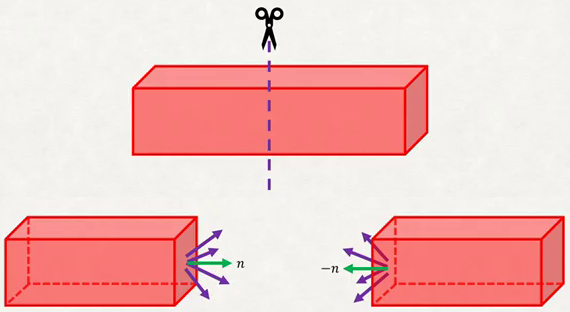
\includegraphics[width=20em]{phy_020_strs_02_01.png}

Kesit düzleminden bahsedelim önce, kesit tam dik olabilir ama bu şart değil,
nasıl olursa olsun o düzleme dik olan bir $\vec{n}$ vektörü ile bu kesitin
duruşunu temsil edebiliriz. 

Bu serbest bırakılmış iç kuvvetler darmadağın gözüküyor. Bir $\Delta A$
alanı tanımlayıp o alandaki tüm kuvvetleri alıp toplarsak bir $\Delta F$
elde edebiliriz, bu tek vektör daha derli toplu.

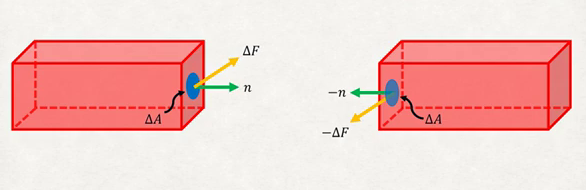
\includegraphics[width=20em]{phy_020_strs_02_02.png}

$\vec{n}$ ile tanımlı bir nokta etrafındaki düzlemin çekiş vektörünü (yani bir
noktadaki stres vektörü) şimdi şöyle tanımlıyoruz,

$$
t_n = \lim_{\Delta A \to 0} \frac{\Delta F}{\Delta A}
$$

Newton'un hareket kanunu üzerinden tabii ki sol taraftaki çekiş ile sağ
taraftaki birbirini dengelemeli, $t_n = -t_{-n}$.

Çekiş vektörü için formel tanım böyle. Ama kimse formel tanımı pek sevmiyor
sözel şekilde anlatırsak, çubuğu aldım ve kestim, Statik dersi der ki kaykılma
(shear), normal kuvvet ve eğilme momentimi böylece elde ederim. Bu üç boyutlu
nesnelerde olan şudur, çubuğu kesiyorum ve bileşenleri stres öğeleri olan tek
bir vektör elde ediyorum.

Şimdi çekiş vektörü kavramını daha basitleştirmeye uğraşalım. Bunun için
patatesimize geri dönüyoruz. Patatesten üç boyutlu sonsuz küçük küp şeklinde bir
parça çıkarttığımızı düşünelim şimdi,

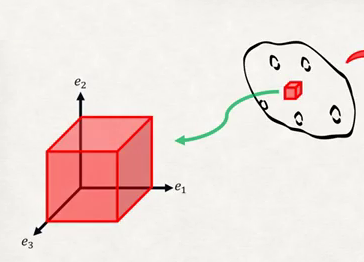
\includegraphics[width=15em]{phy_020_strs_02_03.png}

Bu ufak parça nesnenin bütünlüğünden çıkartıldığı için çekiş vektörlerinin
bu küpün yüzlerine etki eden stres vektörleri olduğunu söyleyebiliriz.

Küp sekli iyi bir seçim aslında çünkü her yüz kordinat eksendeki bir baz düzleme
paralel. Ayrıca $t_{e_1}$, $t_{e_2}$, $t_{e_3}$ yerine de daha iyi bir temsil
şekli bulabiliriz, küpün her yüzündeki bu $t$ çekiş vektörlerini de üç parçaya
ayırabiliriz,

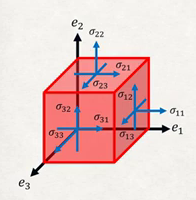
\includegraphics[width=10em]{phy_020_strs_02_04.png}

Bu şekildeki temsilin iyi bir tarafı her yüzdeki üç vektörün orijindeki
baz vektörlerle birebir uyuşması. O zaman mesela $t_{e_3}$'u o baz vektörlerin
lineer bir kombinasyonu olarak yazabilirim,

$$
t_{e_3} = \sigma_{31} e_1 + \sigma_{32} e_2 + \sigma_{33} e_3
$$

Üsttekini herhangi bir yüzey için yazarsak, yani $e_i$'in dik olduğu bir yüzey
için

$$
t_{e_i} = \sigma_{ij} e_j
$$

Einstein notasyonu kullandık, bu notasyonla her $i$ için mümkün tüm $j$'lerin üç
tane terimi ortaya çıkardığı kabul edilir.

Küpün yüzlerindeki çekiş vektörünü gösterebiliyoruz, fakat acaba herhangi bir
yöne bakan bir yüzey için stres vektörü ne olurdu? Bu ifadeyi genel bir şekilde
yazmak mümkün, hem bunu göstermek (ve ileride ispat etmek) için Cauchy Stres
Tetrahedon'u denen bir kurguyu anlatmamız lazım.

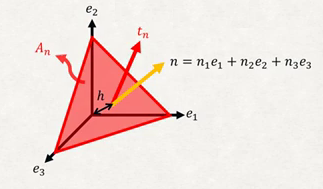
\includegraphics[width=20em]{phy_020_strs_02_05.png}

Tetrahedon üstteki gibi tanıdık bir şekil. Cauchy Lemma'sı ve Cauchy Kanununa
göre

$$
t_n = \sigma^T n
$$

olarak belirtilebilir, detaylı olarak belirtirsek,

$$
\left[\begin{array}{ccc}
t_{n1} \\ t_{n2} \\ t_{n3} 
\end{array}\right] =
\left[\begin{array}{ccc}
\sigma_{11} & \sigma_{21} & \sigma_{31} \\
\sigma_{12} & \sigma_{22} & \sigma_{32} \\
\sigma_{13} & \sigma_{23} & \sigma_{33} 
\end{array}\right]
\left[\begin{array}{ccc}
n_1 \\ n_2 \\ n_3
\end{array}\right]
$$

Bu formüldeki $\sigma$ Cauchy stres tensörü olarak adlandırılır. Üstteki ifade
şunu söylemiş oluyor aslında, üstünde kuvvet etkileri olan bir katı cisim bize
verilince yönden bağımsız bir Cauchy stres tensörü $\sigma$ elde edebiliriz,
yani öyle bir $\sigma$ vardır ki $n$ yönündeki $t_n$ elde etmek için
$t_n = \sigma^T n$ yapılabilir.

Cauchy tensörü hakkında bazı ispatlar için [1, sf. 330]. 

Cauchy tensörünün bazı özellikleri,

1) $\sigma$ simetriktir, yani $\sigma_{ij} = \sigma_{ji}$.

2) Öyle bir kordinat sistemi vardır ki bu sistemde $\sigma$ köşegendir. Lineer
cebirde köşegenleştirme vardır bildiğimiz gibi, burada o teknik uygulanır, bu
şekilde asal stresleri (principle stresses) denen stres vektörleri elde
edilebilir.

3) Feragat / teslim / esneme yüzeyi (yield surfaces) denen bir hesabı bu tensör
üzerinden yapmak mümkün. 

Normal ve Kaykılma Stresleri

Çekiş vektörü kavramının bir daha üzerinden geçelim, formülü gördük ama
kavramsal olarak neyden bahsediyoruz? İki boyuttaki kütleye bakalım, onu
herhangi bir düzlemle kestim diyelim, 

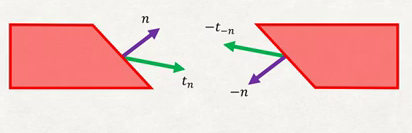
\includegraphics[width=15em]{phy_020_strs_02_06.png}

Kesim yüzeyini normal vektörü ile tanımlıyoruz. Çekiş vektörü bir objenin iç
streslerinin bir yüzeye yansımasıdır. Dikkat, bu iç streslerin, kuvvetlerin
vektörsel bileşimleri illa ki yüzeyin normal vektörü ile aynı yönde olmayabilir,
onun için üstteki şekilde farklı yöne bakan bir $t_n$ gösteriliyor. Muhakkak
diğer parçada ona eşit dengeliyici reaksiyon var, vs.

Şimdi çekiş vektörünün bileşenlerine gelelim, $t_n$ daha önce belirttik stres
tensoru çarpı $n$. 

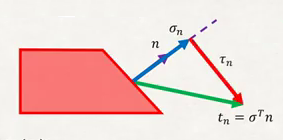
\includegraphics[width=10em]{phy_020_strs_02_07.png}

Bileşen bağlamında $t_n$'i alıp $n$ üzerine skalar olarak yansıtabilirim,
$\sigma_n$ büyüklüğünü elde ederim, ona normal stres diyelim. Bu bir skalar
büyüklük, hesabı

$$
\sigma_n = \proj_n t_n = \frac{t_n \cdot n}{||n||}
$$

Üstteki hesap aslında daha da basitleşebilir çünkü $n$'nin norm'u 1'e
eşittir yani $||n||=1$, o zaman geriye sadece $\sigma_n = t_n \cdot n$
kalıyor.

Yüzeye paralel olan bileşen kaykılma stresi (resimde kırmızı renkli $\tau_n$)
için artık basit bir vektör çıkartım işlemi yeterli, resme göre

$$
t_n = \vec{\sigma}_n + \vec{\tau}_n 
$$

olduğuna göre basit bir tekrar düzenleme sonrası,

$$
\vec{\tau}_n  = \vec{t}_n - \vec{\sigma}_n 
$$

elde edilir. Yanlız $\vec{\sigma}_n$ vektörü kullanıldı, daha önce $\sigma_n$
skalar demiştik, vektörü nasıl elde ediyoruz? Bu basit, $\vec{\sigma}_n$
yönsel olarak normal vektör $n$, ya da $\vec{n}$ ile aynı yönde olacağı
için, eh $\vec{n}$ zaten birim vektördür o zaman $\vec{\sigma}_n$ için
$\vec{n}$ ile $\sigma_n$ çarpılması yeterli,

$$
\vec{\tau}_n  = \vec{t}_n - \sigma_n n
$$

Asal Stresler

FEM programlarında karşımıza çıkan bir kavram bu. Eğer $\sigma$ simetrik ise
stres tensörünün özvektörleriyle eş olan öyle bir kordinat sistemi vardır ki bu
sistemde stres tensörü köşegen haline gelir (kaykılma stresi kalmaz). Bu bir
köşegenleştirme operasyonu aslında.  Daha önce üzerinde stres öğeleri olan küpü
göstermiştik, köşegenleştirme ile yapılan bu küpü öyle bir çevirmek ki kaykılma
bileşeni kalmasın.

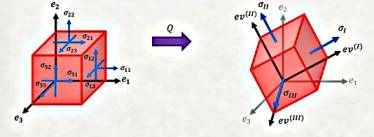
\includegraphics[width=20em]{phy_020_strs_02_08.jpg}

$Q$ vektörü stres tensörünün özvektörlerinden oluşuyor, 1'inci özvektör $Q$'nun
1'inci satırına ikinci özvektör ikinci satırına, vs. Bu Lineer Cebirden
bildiğimiz köşegenleştirme operasyonu tabii ki, yapmaya uğraştığımız $\sigma$'yi
köşegenleştirip bir $\sigma'$ elde etmek,

$$
\sigma = 
\left[\begin{array}{ccc}
\sigma_{11} & \sigma_{21} & \sigma_{31} \\
\sigma_{12} & \sigma_{22} & \sigma_{32} \\
\sigma_{13} & \sigma_{23} & \sigma_{33} 
\end{array}\right] \implies
\sigma' = Q \sigma Q^T =
\left[\begin{array}{ccc}
\sigma_I & 0           & 0 \\
0        & \sigma_{II} & 0 \\
0        & 0           & \sigma_{III}
\end{array}\right]
$$

ki $\sigma_I$, $\sigma_{II}$, $\sigma_{III}$ $\sigma$'nin özdeğerleridir, elde
edilen özdeğerler büyükten küçüğe doğru sıralanır, $\sigma_I > \sigma_{II} > \sigma_{III}$
olacak şekilde.

[atlandı]

Belirleyici Kanun (Constitutive Law), Stres-Gerilme İlişkisi

Şimdiye kadar stres tensoru $\sigma$ ve gerilme tensoru $\epsilon$ hakkında
öğrendiklerimizi kullanarak ikisi arasında bir ilişki [2, 1:15:50] kurabilir
miyiz acaba?

[atlandı]

Euler-Bernoulli Kirişleri (Beams)

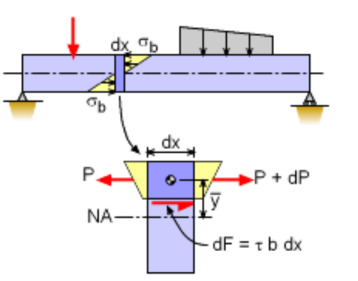
\includegraphics[width=20em]{phy_020_strs_02_09.jpg}

Mühendislikte, özellikle inşaat mühendisliğinde kirişler yaygın bilinen
bir konudur. Bir kiriş bağlamında

\begin{itemize}
   \item Kaykılma Kuvvet Fonksiyonu $V(X_1)$
   \item Bükülme Moment Fonksiyonu $M(X_1)$
   \item Saptırma (Deflection) Fonksiyonu $y(X_1)$
\end{itemize}

gibi kalemlerle ilgileniyor olabilirim. Bu kalemlerden ilk ikisi çok basittir.
Üçüncü hesap mesela kirişin ``servis edebilir'' olup olmadığını söyleyebilir
mesela, ki insanlar bu kirişin üstünde yürüdüğünde oraya buraya savrulmasınlar
(saptırma bu hesabı bize verebilir). İşte üstteki türden hesapları yapabilmek
için Euler-Bernoulli kiriş faraziyesinden yola çıkmak yaygın bir yaklaşımdır.
Bu faraziyeler nelerdir? 

\begin{itemize}
   \item Deformasyonlar ufak: Bu doğal bir varsayım, inşaat mühendisliğinde
     mesela eğer ortada bir deprem yok ise çok büyük şekil değişiklikleri
     beklemeye gerek yok. 
   \item Kiriş lineer elastik esyonlu maddeden yapılmış: inşaat
     mühendisliğindeki çelik kirişlerin zaten böyle olduğu farz edilir.     
   \item Poisson oranı etkileri yoksayılır.
   \item Düzlem bölümler düzlem kalır. Boyu eninden cok daha fazla olan
     nesnelerde bu dogrudur, fakat daha ufak parcalarda varsayim tutmayabilir.
\end{itemize}

İç Kuvvetler - Kaykılma ve Bükülme Momenti

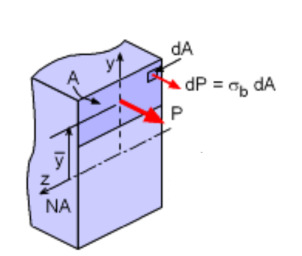
\includegraphics[width=30em]{phy_020_strs_02_10.jpg}

Kirişin ufak bir bölümüne odaklanıyoruz ve oradaki kuvvetleri listelemeye
uğraşıyoruz. Üstte birinci resimdeki parçaya bakıyoruz, $\ud X_1$ genişliğinde,
ve üzerinde dağıtık yük $q$ var. Unutmayalım bir parçayı kesip çıkartınca onun
üzerindeki kuvvetler hayali olarak ortaya ``saçılır'', bu saçılma çekiş
vektörleri kadar çetrefil değil muhakkak (çünkü faraziyelerle pek çok şeyi
burada basitleştirdik) ama üç tane temel kuvvet olduğunu biliyoruz.

Kuvvetlerden ilki üstteki resimde soldan birinci, normal kuvvet $N$. Bu kuvvet
parçanın sol tarafında $N$, sağ tarafında $N$'deki ($X_1$'e göre) değişim çarpı
$X_1$'deki değişim. Aynı parçayla ve resimle devam ediyoruz, soldan ikinci
resimde kaykılma kuvveti $V$ var, aynı değişim matematiği orada da var, ve
nihayet soldan üçüncü resimde bükülme momenti, benzer matematik.














Ekler

Giriş dersinden hatırlarsak kuvvet uygulanan çubuklardaki deformasyon maddenin
özellikleriyle ilişkilendirilebiliyordu, bunun için birim alandaki kuvvet ve
birim boya tekabül eden uzama gözönüne alınıyordu. Çok boyuta geçerken ilk
olarak birim alan bazlı içsel kuvvetlerin alttaki gibi genel bir nesneye
nasıl uygulanacağını görelim [3, sf. 184].

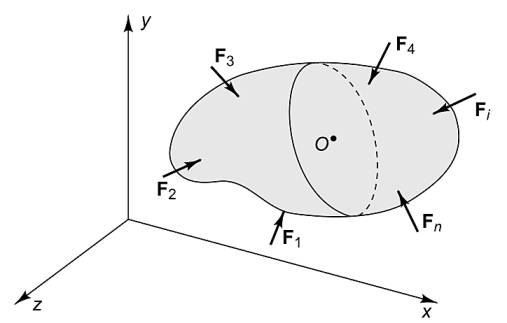
\includegraphics[width=15em]{phy_020_strs_02_app_01.jpg}

Bir $O$ noktasına etki eden iç kuvvetleri incelemek için o noktadan geçen bir
düzlem hayal edebiliriz, düzlemi temsil eden ona dik normal vektör $n$ olsun.
Eğer düzlemi ufak parçalara bölsek ve her bölgeye etki eden kuvvetleri ölçsek
oradaki etki eden kuvvetlerin birinden diğerine değişebileceğini görürdük.

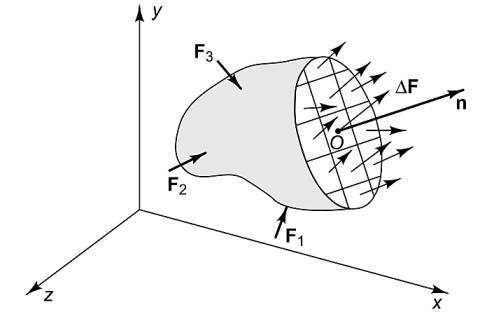
\includegraphics[width=15em]{phy_020_strs_02_app_02.jpg}

Eğer benzer şekilde $O$ merkezli bir ufak kare $\Delta A$ ele alsak orada etki
eden bir $\Delta F$ olacaktır. $\Delta F$'nin düzleme dik olması gerekmez,
herhangi bir açıda duran bir vektör olabilir, cismin altındaki kuvvetler üstten
alta doğru bastıran kuvvetlerden daha büyükse $\Delta F$ onların tek bir
noktadaki bir tür birleşimi olduğu için yukarı doğru gösteriyor olurdu muhakkak.

Şimdi stres vektörü kavramını tanıştıralım; eğer $\Delta A$ limite doğru giderse

$$
T_n = \lim_{\Delta A \to 0} \frac{\Delta F}{\Delta A}
$$

büyüklüğü stres vektörünü tanımlar.

Dikkat edersek $\Delta F$ büyüklüğü düzlemin duruşuna, yani $n$'ye bağlı olduğu
için özellikle $n$ ibaresini $T$ sembolüne ekledik; her değişik $n$ değişik bir
$T_n$ değerini verebileceği için.

Herhangi bir düzlem kullanabiliriz demiştik, fakat tekrarlanabilirlik, net
ifade açısından her eksene dik birer düzlem, toplam üç tane kullanmak daha
iyi olabilir. Mesela $x$ eksenine dik olan bir düzlem altta,

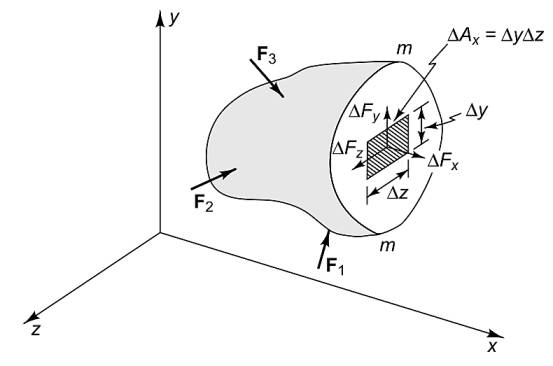
\includegraphics[width=20em]{phy_020_strs_02_app_03.jpg}

Daha önce gördüğümüz $\Delta F$'in üstteki resimde düzleme göre bileşenlerine
ayıracağız, bunlar $\Delta F_x$, $\Delta F_y$, $\Delta F_z$. Baktığımız alan ise
kenarları $\Delta y$ ve $\Delta z$ olan bir dikdörtgen, alan $\Delta A_x$ ise
(notasyon olarak dik olduğumüz eksenin sembolünü verdik)
$\Delta A_x = \Delta y \Delta z$.

Daha önce olduğu gibi burada da limit tekniğini kullanabiliriz, $\Delta A_x \to
0$ olacak. Fakat yine notasyonel olarak referans eksen yönündeki strese $\sigma$
sembolü üzerinden normal stres , o eksene dik yani düzleme paralel olan
bileşenlere $\tau$ üzerinden kaykılma (shear) stresi adlarını vereceğiz.
Limitlerle beraber,

$$
\sigma_x = \lim_{\Delta A_x \to 0 } \frac{\Delta F_x}{\Delta A_x}
$$

$$
\tau_{xy} = \lim_{\Delta A_x \to 0 } \frac{\Delta F_y}{\Delta A_x}
$$

$$
\tau_{xz} = \lim_{\Delta A_x \to 0 } \frac{\Delta F_z}{\Delta A_x}
$$

Aynı düzlemle kesme tekniğini iki diğer eksen $y,z$ için de kullanırsak, ve
benzer hesapları yaparsak oradan da altı tane stres değeri elde ederiz, toplam
dokuz tane, hepsi bir arada bir matris içinde,

$$
\left[\begin{array}{rrr}
\sigma_x & \tau_{xy} & \tau_{xz} \\
\tau_{yx} & \sigma_y & \tau_{yz} \\
\tau_{zx} & \tau_{zy} & \sigma_z
\end{array}\right]
$$








[devam edecek]

Kaynaklar

[1] Kelly, Solid Mechanics Part III, Auckland University

[2] Petitt, {\em Intro to the Finite Element Method}, University of Alberta,
    \url{https://www.youtube.com/watch?v=2iUnfPRk6Ro&list=PLLSzlda_AXa3yQEJAb5JcmsVDy9i9K_fi}

[3] Crandall, {\em An Introduction to the Mechanics of Solids}

\end{document}
